
\newcommand{\citeauthorandyear}[2][]{
   [\citeauthor{#2} (\citeyear[#1]{#2})]
}

\documentclass[12pt]{article}

\usepackage{graphicx} % Required for inserting images
\usepackage[left=1.5in, right=1.2in, top=1.2in, bottom=1.2in]{geometry}
\usepackage{url}
\usepackage{amsmath}
\usepackage{cleveref}
\usepackage{indentfirst}
\usepackage[backend=biber, style=authoryear-ibid]{biblatex}
\usepackage{siunitx}
\usepackage{mathptmx}
\usepackage{setspace}



\renewcommand*{\bibfont}{\footnotesize}
\renewcommand{\refname}{\fontseries{m}\selectfont References}
\addbibresource{bibliography.bib}

\def \projectname {Review on Gravitational Wave Analysis of Neutron Stars}
\def \authone {V. Dheeraj Shenoy}
\def \authtwo {Aprameya M. Haritsa}
\def \guidename {Mr. Sundar M. N.}
\def \director {Dr. Asha Rajiv}
\def \mdot {$M_\odot$ }

\linespread{1.5} % Set line spacing to 1.5 times

\begin{document}

\begin{center}

\thispagestyle{empty}


\includegraphics[width=0.4\textwidth, height=0.12\textwidth, ]{images/jain logo.png}

\vspace{1cm}

\textbf{\huge{{\projectname}}}

\vspace{0.7cm}

\Large{Submitted By}

\vspace{0.3cm}

\textbf{\large{\authone}}\\
\textbf{\normalsize{USN: 22MSRPH022}}

\vspace{0.5cm}

\textbf{\large{\authtwo}}\\
\textbf{\normalsize{USN: 22MSRPH019}}

\vspace{0.75cm}

\Large{Under the Guidance Of}

\textbf{\large{\guidename}}

\vspace{0.75cm}

To

\vspace{0.4cm}

\large

Department Of Physics and Electronics \\
School Of Sciences, JAIN (Deemed-to-be University)\\
Bengaluru\\

\vspace{1cm}

\textbf{\large{June 2023}}

\end{center}

\newpage

% CERTIFICATE PAGE

\thispagestyle{empty}

\begin{center}


\includegraphics[width=0.4\textwidth, height=0.12\textwidth, ]{images/jain logo.png}

\large
\vspace{1cm}

\textbf{Department Of Physics and Electronics\\
School Of Sciences, JAIN (Deemed-to-be University)\\
Bengaluru.}

\vspace{1cm}

\underline{\textbf{CERTIFICATE}}

\end{center}

\vspace{0.5cm}

\normalfont{}
\noindent
This is to certify that the plan of the present project titled ``\textbf{\projectname}" has been the outcome of an original study carried out by \textbf{\authone} and \textbf{\authtwo} under the supervision of \textbf{\guidename} towards the partial fulfilment of the requirements for the degree of M.Sc. Physics of JAIN (Deemed-to-be University).

\vspace{0.5cm}

\noindent
This to further certify that the work reported herein does not form a part of any other thesis/dissertation, on the basis of which a degree, diploma or a certificate has been conferred upon this or any other student in the past.

\vspace{3cm}

\noindent
\begin{minipage}{0.5\textwidth}

\textbf{\director}

Director\\
School Of Sciences\\
JAIN (Deemed-to-be University)\\
Bengaluru

\end{minipage}%
\begin{minipage}{0.5\textwidth}
\textbf{\guidename}

Project Supervisor\\
Deparment of Physics and Electronics\\
JAIN (Deemed-to-be University)\\
Bengaluru
\end{minipage}

% DECLARATION

\thispagestyle{empty}

\begin{center}
\Large

\underline{\textbf{DECLARATION}}\\

\end{center}

\vspace{1.5cm}

\noindent
We, \textbf{\authone{}}, \textbf{\authtwo{}} hereby declare that this dissertation titled \textbf{\projectname} has been the outcome of an original study carried out under the guidance of \textbf{\guidename} towards
the partial fulfilment of the M.Sc. Physics degree of the JAIN (Deemed-to-be University)
during the year 2023-2024. This study has not been submitted for any degree, diploma or
certificate.

\vspace{5cm}

\noindent
\begin{minipage}{0.5\textwidth}
\flushleft
(\authone)

\vspace{1.5cm}

(\authtwo)

\end{minipage}%
\begin{minipage}{0.5\textwidth}
\flushright

\textbf{June, 2023\\
Bengaluru}
\end{minipage}
% ACKNOWLEGDEMENTS

\thispagestyle{empty}

\begin{center}

\Large{\underline{\textbf{ACKNOWLEDGEMENT}}}\\

\end{center}

\vspace{1cm}

\noindent
We would like to express our sincere gratitude to \textbf{\guidename} for his invaluable guidance and support throughout our project. His expertise has been instrumental in our success. We are truly grateful for his contributions and the knowledge we have gained under his mentorship.

\vspace{0.5cm}

\noindent
We are also grateful to \textbf{\director}, Director, School of Sciences,
\textbf{Dr. K. N. Varalakshmi}, Director, Centre for Research in Pure \& Applied Sciences and
\textbf{Dr. K. R. Sridhara Murthi}, Director of Academics \& Planning, JAIN (Deemed-to-be
University) for providing us with this opportunity. We are thankful to \textbf{Dr. N. Shanthi},
Head of the Department of Physics and Electronics and \textbf{Dr. S. Thiyagaraj}, Programme-
Head, M. Sc. Programme, for their constant support and encouragement.

\vspace{0.5cm}

\noindent
We thank \textbf{Dr. Chenraj Roychand}, Chancellor, \textbf{Dr. N. Sundararajan},
Pro-Chancellor and \textbf{Dr. Raj Singh}, Vice-Chancellor, JAIN (Deemed-to-be University), for
providing the required infrastructure and support without which this project would not have
been possible.

\vspace{0.5cm}

\noindent
We are grateful to all the faculty members, Mr. Arvind Krishnapur, Physics lab technician and Mr. Rajesh, Physics lab assistant for their kind support towards us.

\vspace{1.5cm}

\noindent
\begin{minipage}{0.5\textwidth}

(\authone)

\vspace{1.5cm}

(\authtwo)

\end{minipage}%
\begin{minipage}{0.5\textwidth}
\flushright

\textbf{June, 2023\\
Bengaluru}
\end{minipage}
% UNDERTAKING FILE

\thispagestyle{empty}

\begin{center}
    
\Large{\underline{\textbf{UNDERTAKING}}}\\


\end{center}

\vspace{1.5cm}

\noindent
We, \textbf{\authone{}}, \textbf{\authtwo{}} hereby give an undertaking that the data
reported in the present dissertation will not be used for any publication, conference
presentation or for any industrial interaction without a written approval from the Project
Supervisor and the Director, School of Sciences, JAIN (Deemed-to-be University).

\vspace{5cm}

\noindent
\begin{minipage}{0.5\textwidth}

(V Dheeraj Shenoy)

\vspace{1.5cm}

(Aprameya M. Haritsa)
\end{minipage}%
\begin{minipage}{0.5\textwidth}
\flushright

\textbf{June, 2023\\
Bengaluru}
\end{minipage}

\thispagestyle{empty}
\tableofcontents

\newpage

% SECTION : ABSTRACT
\setcounter{page}{1}

    
\begin{center}
    \large{\textbf{Abstract}}
\end{center}

\noindent
Most dense star in the universe is neutron star. We discuss here briefly the formation of neutron stars and their types, and then gravitational wave analysis. We discuss the challenges that are involved in gravitational wave analysis of neutron stars particularly magnetars, and how it can be analysed to understand the processes involved in the formation of these peculiar stars. We discuss the sensitivity of the current gravitational wave detectors. The magnetic fields of neutron stars are a crucial aspect of their nature, and their origin and influence are explored in detail. The paper discusses various mechanisms for the generation and amplification of magnetic fields in neutron stars, including the role of progenitor stars and dynamo processes. The immense strength of neutron star magnetic fields and their impact on the star's structure, radiation emission, and surrounding environment are also addressed. We cover the detection of neutron stars through pulsar observations, X-ray and gamma-ray emission, and gravitational wave signals. The paper also discusses the exploration of highly magnetized neutron stars known as magnetars and their unique phenomena, such as bursts and flares.\\

\noindent
\textbf{Keywords}: Neutron stars, Magnetars, Pulsars, Black Widow pulsars, Gravitational Wave, Relativity, Gamma Ray Burst, Flares, Event Rate, Continuous Gravitational Waves.


\newpage

\section{Introduction}

% INTRODUCTION

\normalsize

In the vast tapestry of the cosmos, where celestial bodies of various sizes and compositions populate the universe, neutron stars stand out as extraordinary phenomena. These enigmatic objects, born from the violent deaths of massive stars, are the remnants of stellar evolution pushed to the brink of collapse. Neutron stars are captivating not only due to their extreme physical properties but also because they provide a unique window into the fundamental laws of physics operating in the most extreme environments imaginable.\\

In 1934, two astronomers, Baade and Zwicky, in their paper \citeauthorandyear{baade_zwicky} hypothesized the existence of neutron stars as an ultimate fate of any ordinary star once their nuclear fuels are exhausted. This came shortly after the hypothesis of existence of neutron by James Chadwick  \citeauthorandyear{james_chadwick} in 1932. In 1967, Jocelyn Bell, a postgraduate student working under Anthony Hewish, \citeauthorandyear{bell_hewish}, discovered a star that was pulsating, which later came to be known as pulsars, which is a type of neutron star.\\

Neutron stars, despite their name, are not composed solely of neutrons. Rather, they consist of an unimaginably dense and compact core formed predominantly by tightly packed neutrons. This exotic state of matter, known as neutronium, arises under the immense gravitational forces that act upon the collapsing stellar core during the supernova explosion. The resulting neutron star boasts an average mass comparable to that of our Sun but compressed into a sphere with a radius on the order of only a dozen kilometers. Such extraordinary densities give rise to mind-boggling physical phenomena, making neutron stars a playground for scientists to explore the frontiers of physics.\\

\newpage
Neutron stars exhibit a diverse range of fascinating behaviors and emit various forms of electromagnetic radiation across the electromagnetic spectrum. Pulsars, a type of rapidly spinning neutron star, emit regular beams of radio waves, creating a lighthouse-like effect as the beams sweep across our line of sight. These ``cosmic beacons" have become valuable tools for probing the underlying physics of neutron stars and for studying the properties of interstellar matter and magnetic fields.\\

Furthermore, neutron stars are involved in extreme astrophysical events, such as supernova explosions and binary star mergers. These cataclysmic events release vast amounts of energy and generate powerful phenomena like gamma-ray bursts and gravitational waves. By studying the aftermath of such events, scientists can deepen their understanding of the physical processes that govern the universe and gain insights into the formation of heavy elements, like gold and platinum.\\
\newpage

\section{Formation of a Neutron Star}


When the nuclear fuel in a star is exhausted, the gaseous clouds start to collapse under the gravitational pull and explodes in a supernova event. After supernova, only a fraction of the mass is left, and the final product might be a white dwarf, a neutron star or a black hole, depending on the mass of the progenitor. If the collapsing core is about 8 - 25 \mdot, where \mdot is the solar mass $\approx \num{2e33}$ g, the electrons and protons in the gaseous cloud get converted to neutrons under high pressure to form a neutron star. Further collapse is prevented by neutron degeneracy pressure, a phenomenon described by the Pauli Exclusion Principle. If the mass of the neutron star formed is in excess of 2 - 3 \mdot the mass is greater than the above mentioned limit then it leads to the formation of a black hole.\\

Neutron stars are characterized by their high densities, typically around 1.4 to 2 times the density of atomic nuclei. This extreme density is responsible for their unique properties and behaviors. The neutrons in the core are packed so tightly that they interact strongly with each other, giving rise to a state of matter called neutronium. Neutron stars possess incredibly strong gravitational fields, which warp the surrounding spacetime and create gravitational wells.\\

The formation of a neutron star is a violent and energetic process, releasing an enormous amount of energy in the form of neutrinos and a supernova explosion. These explosions contribute to the dispersal of heavy elements and enrich the interstellar medium with the products of nucleosynthesis.\\

In recent years, the detection of gravitational waves from neutron star mergers has provided additional insights into their formation. When two neutron stars in a binary system spiral inward due to the emission of gravitational waves, they eventually collide and merge. This merger event releases a tremendous amount of energy in the form of gravitational waves, gamma-ray bursts, and other electromagnetic radiation, leading to the formation of highly massive neutron stars or even black holes.\\

The formation of neutron stars is a captivating process that highlights the incredible forces and extreme conditions present in the universe. The study of neutron star formation not only expands our knowledge of stellar evolution but also provides a deeper understanding of the fundamental physics governing matter at extreme densities and temperatures.\\

\begin{figure}[h]
\centering
\includegraphics[height=0.9\textwidth, width=0.9\textwidth]{images/Neutronstarsimple.png}
\caption{\small Simplified representation of the formation of neutron stars credits; Bedrock Person; 22 June 2017}
\end{figure}

\newpage
\section{Properties of Neutron Star}

\subsection{Radius}

The radius of a neutron star is typically on the order of 10 to 15 kilometers \citeauthorandyear{kutschera1998neutron}, making them incredibly compact objects. To put this into perspective, neutron stars have a radius that is about 1,000 times smaller than the radius of the Earth and only about 10 kilometers across.\\

The exact radius of a neutron star depends on its mass, composition, and equation of state, which describes the relationship between density, pressure, and other properties of the stellar matter. Neutron stars with higher masses tend to have slightly smaller radii due to the stronger gravitational forces. A maximum limit for the radius of neutron stars have been found out to be between 10.4 - 11.9 km \citeauthorandyear{Capano2020}\\

The determination of the radius of a neutron star is a challenging task and requires sophisticated modeling and observational techniques. Indirect methods, such as analyzing the X-ray spectra and thermal emission from the surface of neutron stars, can provide valuable insights into their radius. Additionally, multi-wavelength observations, such as the study of gravitational waves from neutron star mergers, can help constrain the radius and other properties of neutron stars.\\

It is important to note that the concept of the ``surface" of a neutron star is not well-defined, as the outer layers of a neutron star can consist of a solid crust, a liquid layer, and a gaseous atmosphere. The structure and composition of these layers can vary depending on the mass and age of the neutron star \citeauthorandyear{kayanikhoo2023maximum}.\\

\subsection{Magnetic Fields}

Magnetic fields in neutron stars are incredibly strong, making them some of the most powerful magnetic fields known in the universe. Neutron stars possess magnetic fields ranging from approximately \num{e8} to \num{e15} Gauss (G), with the higher end of the range representing magnetars, a special class of highly magnetized neutron stars. The origin and strength of the magnetic fields in neutron stars are still active areas of research, but there are several proposed mechanisms for their formation. One theory suggests that the magnetic fields of neutron stars are remnants of the magnetic fields of the progenitor stars. As the massive star undergoes a supernova explosion and collapses, its magnetic field gets amplified due to the conservation of magnetic flux, leading to the formation of a highly magnetized neutron star.

Another possibility is the "dynamo mechanism," which involves the generation and amplification of magnetic fields through various fluid and plasma processes occurring in the core of the neutron star. These processes can be driven by the rapid rotation of the neutron star and the convection of charged particles in its interior.\citeauthorandyear{duncan_thompson}

\subsection{Density}
The density of neutron stars is one of their most remarkable and defining characteristics. Neutron stars are incredibly dense, packing a tremendous amount of mass into a relatively small volume. The density of a neutron star is typically on the order of \num{e17} to \num{e18} kilograms per cubic meter, which is several orders of magnitude greater than the density of atomic nuclei.\\

To put this into perspective, the density of an atomic nucleus is around \num{e17} kilograms per cubic meter, and the density of ordinary matter on Earth is approximately \num{e3} kilograms per cubic meter. Thus, the matter in a neutron star is packed so tightly that it is denser than any known form of matter on Earth.\\

The high density of neutron stars arises from the tremendous gravitational forces present within these compact stellar remnants. The gravitational collapse during the formation of a neutron star compresses the matter to such an extent that the electrons and protons in atomic nuclei combine to form tightly packed neutrons. This neutron-rich matter becomes so dense that it surpasses the densities observed in atomic nuclei.\\

The exact density of a neutron star depends on several factors, including its mass and radius. Typically, neutron stars have masses around 1.4 times that of the Sun, but their radii are only about 10 to 15 kilometers. This compact size, combined with the substantial mass, results in extreme densities.

\subsection{Escape Velocity}
The escape velocity of a neutron star depends primarily on its mass and radius. The mass of a typical neutron star is approximately 1.4 times the mass of the Sun, while its radius is on the order of 10 to 15 kilometers. These values lead to escape velocities of the same magnitude.\\

\noindent
Assuming a mass of 1.4 solar masses (M $\approx \num{2.8e30} kg$) and a radius of 10 kilometers (R $\approx$ 10,000 meters), the escape velocity can be calculated as follows:

\begin{equation*}
    v = \sqrt{\frac{2 M G}{r}}
    = \sqrt{\frac{2 \times \num{2.8e30} \times \num{6.67430e-11}}{10000}}
    = \SI{6.7e7}{\metre/\second}
\end{equation*}

This escape velocity is approximately 0.22 times the speed of light, emphasizing the immense gravitational forces at play near neutron stars. It implies that any object, including light itself, would need to exceed this velocity to escape the gravitational pull and move away from the neutron star indefinitely.\\

\newpage
The high escape velocity of neutron stars has significant implications for their observational properties. It means that the intense gravitational pull can cause substantial gravitational redshift, where the light emitted from the neutron star's surface is stretched to longer wavelengths due to the strong gravitational field. Additionally, it leads to time dilation effects, where time appears to move slower for observers near the neutron star compared to distant observers.\\

Understanding the escape velocities of neutron stars helps us appreciate the immense gravitational forces and extreme conditions present in these objects. The escape velocity acts as a crucial parameter in comprehending the physics and observational aspects associated with neutron stars.

\subsection{Surface Temperature}

The surface temperature of neutron stars varies depending on their age, composition, and thermal evolution. Newly formed neutron stars, known as "hot" neutron stars, can have surface temperatures in the range of millions to tens of millions of degrees Kelvin. However, over time, these temperatures decrease as the neutron star cools and loses thermal energy.\\

The high initial temperatures of neutron stars are a result of their formation processes, particularly the intense energy released during the supernova explosion. During the core collapse and subsequent rebound, a significant amount of energy is generated, contributing to the initial high temperatures of the nascent neutron star.\\

As the neutron star ages, it gradually cools down through a combination of neutrino emission and thermal radiation from its surface. Neutrino cooling dominates in the early stages, as neutrinos, which interact weakly with matter, carry away thermal energy from the star's interior. However, as the neutron star evolves and its interior temperature drops, the rate of neutrino emission decreases, and the surface cooling becomes increasingly important.\\

The cooling process is governed by various factors, such as the composition of the neutron star's crust and core, the presence of magnetic fields, and the rate of energy transfer from the interior to the surface. These factors influence the cooling rate and the final equilibrium temperature reached by the neutron star's surface.\\

Observationally, the surface temperatures of older, "cooled" neutron stars generally range from thousands to hundreds of thousands of degrees Kelvin. These cooler temperatures make them primarily emit thermal X-rays, which are often detected by X-ray telescopes. The exact surface temperature of a neutron star depends on its mass, age, and the efficiency of thermal energy transport mechanisms.\\

It is worth noting that not all neutron stars have the same surface temperature. Neutron stars can exhibit a wide range of temperatures depending on their specific characteristics, such as whether they are isolated or in binary systems, and whether they are accreting matter from a companion star. Factors such as accretion processes, magnetic activity, and the presence of a surrounding atmosphere can significantly influence the observed surface temperature.\\

Determining the precise surface temperature of a neutron star requires detailed observations and sophisticated modeling techniques. Measurements of the thermal radiation emitted by neutron stars across the electromagnetic spectrum, particularly in X-rays, provide valuable insights into their cooling processes and the underlying physics of these exotic objects.\citeauthorandyear{kayanikhoo2023maximum}

\subsection{Rotation Speed}

Neutron stars are known for their incredibly rapid rotation speeds, often referred to as their spin or rotation periods. These rotation speeds can range from milliseconds to several seconds, depending on the individual neutron star. The rapid rotation of neutron stars is a consequence of the conservation of angular momentum during their formation.\\

When a massive star collapses, its core shrinks and conserves its angular momentum, resulting in a drastic increase in rotation speed due to the reduction in size. This phenomenon is similar to an ice skater spinning faster when they pull in their arms.\\

The fastest rotating neutron stars are known as pulsars. Pulsars are highly magnetized neutron stars that emit beams of electromagnetic radiation from their magnetic poles. These beams of radiation are observed as regular pulses of radiation as the neutron star rotates and the beams sweep across our line of sight. Pulsars can rotate hundreds of times per second, with the fastest known pulsar, named PSR J1748-2446ad, rotating at approximately 716 times per second.\\

The rotation speed of a neutron star can be measured using various observational techniques. Pulsar timing is a common method where precise measurements of the arrival times of the pulsar's pulses are made over an extended period. By tracking the timing of these pulses, scientists can determine the rotation period of the neutron star with high precision.\\

The rapid rotation of neutron stars has several important implications. The extreme centrifugal forces due to their fast rotation cause the neutron stars to be oblate or slightly flattened at the poles. Additionally, the high rotational energy of neutron stars can power various astrophysical phenomena, such as the emission of high-energy radiation, the generation of strong magnetic fields, and the production of jets of relativistic particles.\\

In some cases, neutron stars can experience changes in their rotation speed over time. This phenomenon, known as ``glitching", occurs when the neutron star's crust undergoes sudden readjustments, causing a brief increase in rotation speed. Glitches are thought to be caused by the transfer of angular momentum from the superfluid interior of the neutron star to the rigid crust.\\

Understanding the rotation speeds of neutron stars provides valuable insights into their internal structure, magnetic fields, and evolution. It allows scientists to study extreme physical phenomena under the influence of strong gravity and magnetic fields, shedding light on fundamental physics and astrophysical processes.\citeauthorandyear{Heger_2003}

\newpage

\section{Types Of Neutron Star}

There are mainly three classification of neutron star: Pulsar, Magnetar and combination of Pulsar and Magnetar. These classes are further subdivided into other types

\subsection{Pulsars}

The first neutron star to be ever discovered by Jocelyn Bell in 1967 was in fact not just an ordinary neutron star, but was a pulsar. A pulsar is a neutron star star emits electromagnetic radiation from it's magnetic poles. Due to the rotation of the pulsars, the beams appear to be pulsating, similar to a lighthouse. Because their rapid pulse of radio emission is so predictable, a large array of well-understood pulsars can be used to measure extremely subtle abnormalities, such as gravitational waves. Pulsars are used as a timing clock to detect gravitational waves. Knowing the average time required for the pulsar signal to reach earth, the difference between when the pulsar signals should arrive, and when they do arrive, can signal a gravitational wave. A pulsar is depicted in \cref{fig:pulsar_image1}

\begin{figure}[h]
\centering
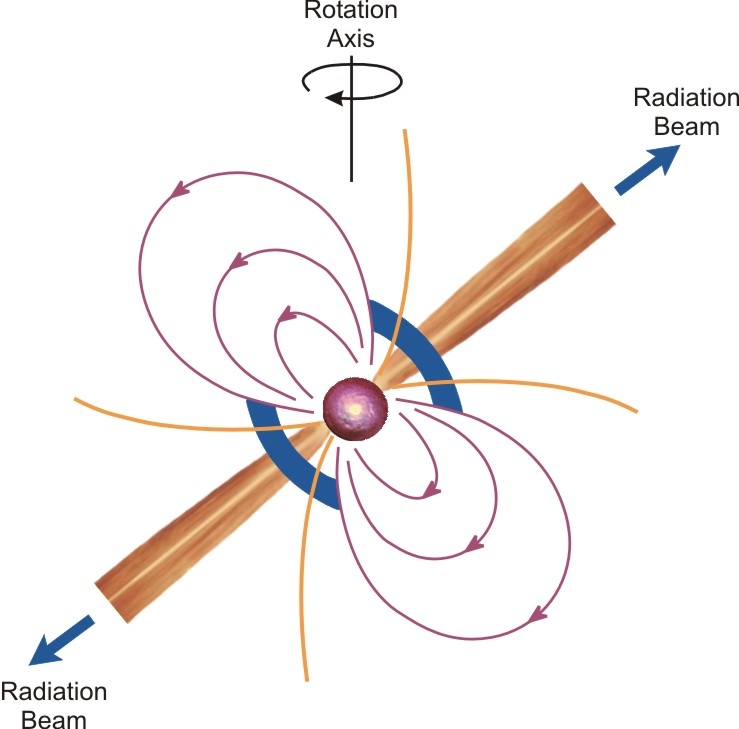
\includegraphics[height=0.5\textwidth, width=0.5\textwidth]{images/pulsar.jpg}
\caption{\small Artistic representation of a Pulsar; Credit: National Radio Astronomy Observatory}
\label{fig:pulsar_image1}
\end{figure}

Pulsars have high magnetic field and as a result, electrons and other subatomic particles are accelerated at very high speeds ($\approx$ the speed of light) causing them to emit beams of radio waves and other forms of radiation. As the pulsar rotates, the radiation beam rotates, and when the beam intersects with earth, we see it.



\subsection{Magnetars}

Magnetars are the neutron stars with unusually high magnetic fields. These have magnetic fields that are almost billion times more stronger than the typical neutron stars. The origin of this very high magnetic field is not full understood, but there have been theories like convective magnetohydrodynamic dynamo effect \citeauthorandyear{duncan_thompson}, or simply as a result of collapse of progenitors having very high magnetic fields. They have been a vast area of research mainly because of their strong magnetic fields of the order of \num{e15} G \citeauthorandyear{pulsar_strong_mag} , and also because they've been known for the cause of Gamma Ray Bursts (GRBs) and X-Ray Bursts (XRBs) and also Fast Radio Bursts (FRBs).\\

\begin{figure}
\centering
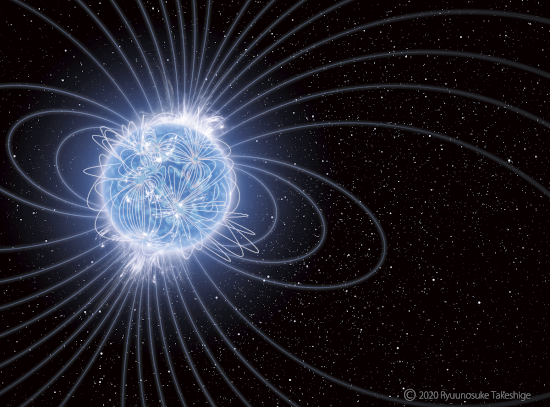
\includegraphics[height=0.5\textwidth, width=0.7\textwidth]{images/magnetar.png}
\caption{\small Artistics image of magnetic lines of a magnetar. Image by Ryuunosuke Takeshige}
\end{figure}

\subsubsection{Magnetars in Binary Systems}

It is still a mystery as to which stars get formed into Magnetars, and which process resulted in the extremely high magnetic field. In \citeauthorandyear{popov_binary_magnetar}, the author discusses the mechanism which might lead to the formation of such a binary system, and various other models that can be used to explain the existence of binary systems having magnetars. Following \citeauthorandyear{where_are_magnetar_binary_companion}, where they've conducted the experiment using photometry method of candidate magnetar counterparts to identify any bound companion stars among the Galactic population, they've estimated that 5 - 10 percent of the galactic population could plausibly have a bound magnetar companion. They've made the estimation assuming that the Magnetars are formed only through core collapse.

\begin{figure}[h]
\centering
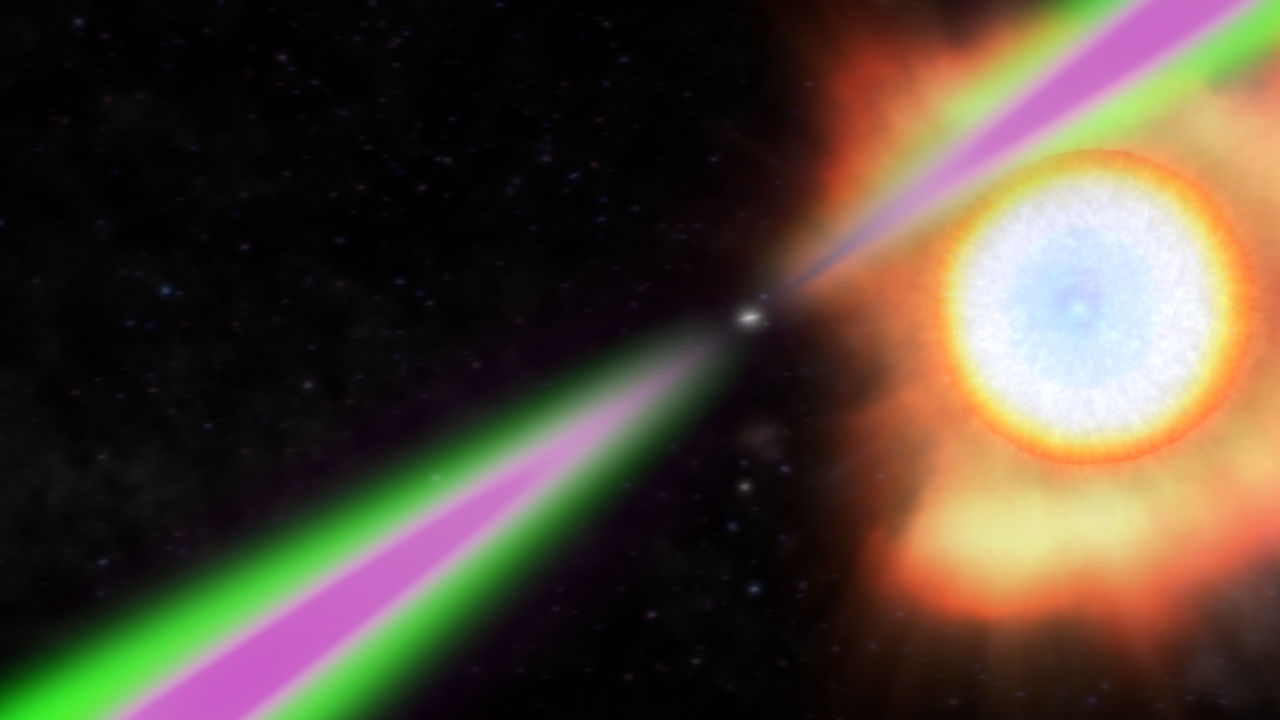
\includegraphics[height=0.4\textwidth, width=0.6\textwidth]{images/BWP.jpg}
\caption{\small Spinning 390 times a second, PSR J1311-3430 periodically swings its radio (green) and gamma-ray (magenta) beams past Earth in this artist's concept. The pulsar heats the facing side of its stellar partner to temperatures twice as hot as the sun's surface and slowly evaporates it. Credits NASA's Goddard Space Flight Center}
\end{figure}

\newpage
\subsubsection{Black Widow Pulsars}

Black widow pulsars (BWPs) are a special class of binary millisecond pulsars (MSPs). Their orbital periods range from 2-20 hours \cite{Formation_BWP_Chen_2013} and  the defining feature of BWPs is theirlow mass companions, with masses much less than 0.1 times of mass of the sun \cite{Bochenek_2015}. Even though BWPs have very small companions, the ionized gas from the companions often eclipses the pulsar. This occurs because the pulsarwind blows stellar material away from the companion, but leaves plasma in the system, creating a screen for the pulsar’s radio emission\cite{Bochenek_2015}.\\

With rotation periods of 10 milliseconds or less, the BWPs spin at very high speeds, upto 43,000 rpm. Today, more than 300 of these millisecond pulsars have been catalogued. Young neutron stars usually appear in isolation, more than half of them have a stellar partner, suggesting that interactions with a normal star can rejuvenate old, slow neutron stars.\\

The intense radiation emitted by the pulsar impacts the companion star, causing it to be heated and partially ablated. This phenomenon earned the Black Widow Pulsar its name, as it metaphorically "consumes" or "destroys" its companion star like a black widow spider consuming its mate. The interaction between the pulsar and its companion has dramatic effects on the companion star. The intense radiation and stellar winds from the pulsar strip away the outer layers of the companion star, creating a trailing gas tail. The process of ablation can lead to the erosion of the companion star's atmosphere and even result in the eventual complete evaporation of the star.



\newpage
\section{Gravitational wave}

Gravitational waves are 'ripples' in space-time caused by some of the most violent and energetic processes in the Universe. Albert Einstein predicted the existence of gravitational waves in 1916 in his general theory of relativity. Einstein's mathematics showed that massive accelerating objects (things like neutron stars or black holes orbiting each other) would disrupt space-time in such a way that 'waves' of undulating space-time would propagate in all directions away from the source. These cosmic ripples would travel at the speed of light, carrying with them information about their origins, as well as clues to the nature of gravity itself.\\

Observations revealed that the orbit of this binary star system was decaying at a rate predicted (to near-perfect precision) by the radiation of gravitational waves due to the orbital motion of the neutron stars. Forty-two years after this initial evidence of their existence, the first direct detection of gravitational waves was announced by the LIGO Virgo Collaborations in 2016.\\

The history of gravitational waves over the century preceding this discovery was at times controversial: from Einstein’s attempt in 1937 to overturn his initial 1916 prediction of their existence; to pioneering, albeit premature, claims of detection by Weber in the 1960s. Seven years on from this historic first discovery, nearly 100 gravitational wave events have been observed, all from colliding binary systems of pairs of black holes (including the first discovery), pairs of neutron stars, or a black hole and a neutron star.\\

\begin{figure}[h]
\centering
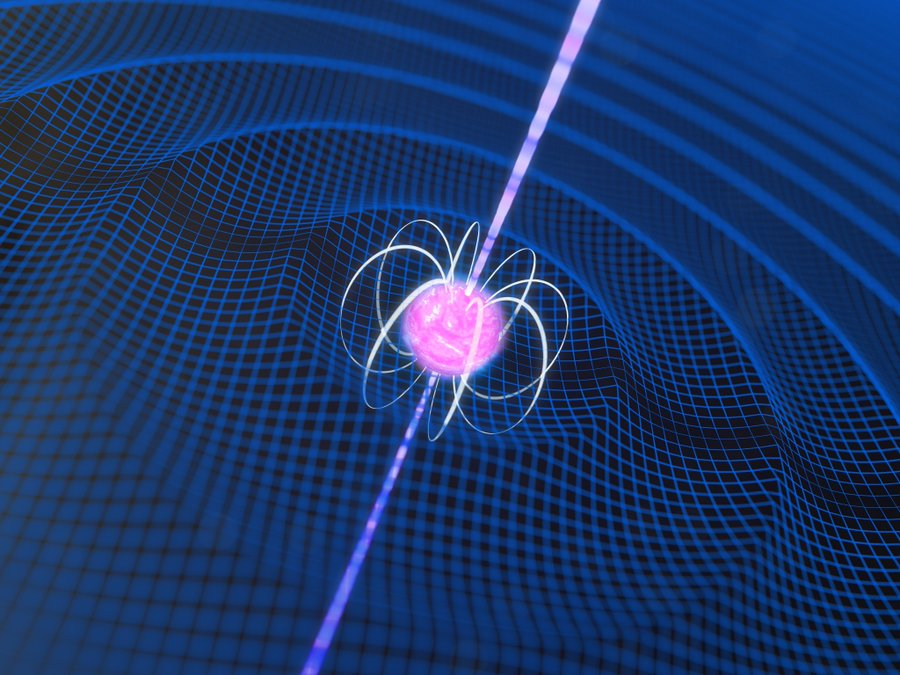
\includegraphics[height=0.4\textwidth, width=0.5\textwidth]{images/Continous gravitational wave.jpg}
\caption{\small Artist’s impression of a neutron star radiating both continuous gravitational waves and electromagnetic radiation. Credit: OzGrav/Carl Knox.}
\end{figure}

\begin{figure}[h!]
\centering
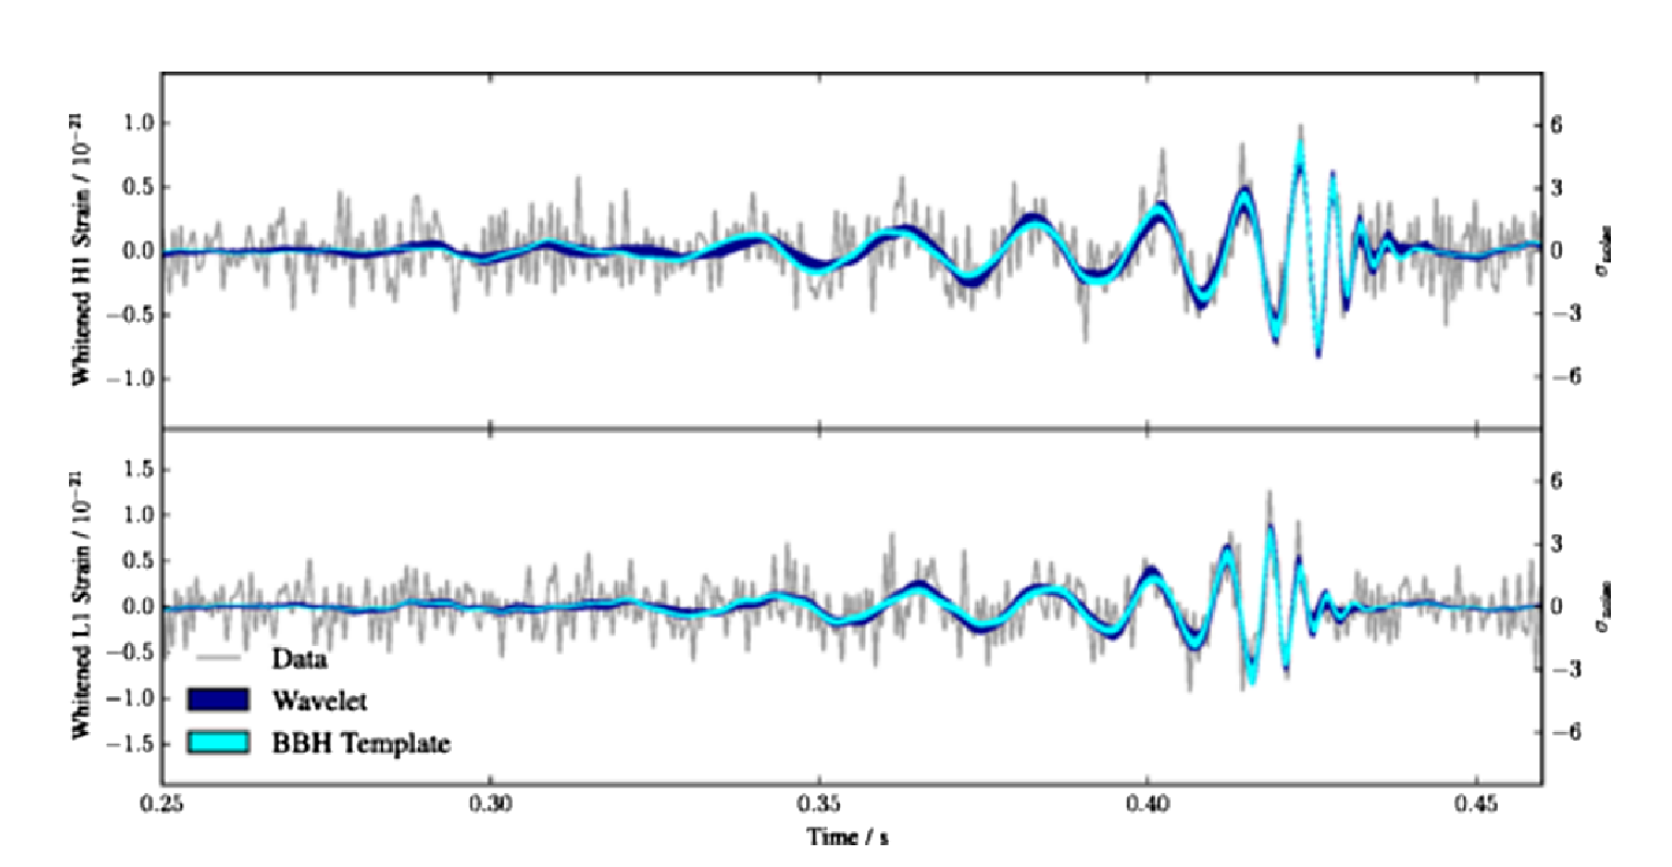
\includegraphics[height=0.7\textwidth, width=0.7\textwidth]{images/mass_estimation_graph.png}
\caption{\small Measured detector strain time series of the first detected gravitational wave signal by Advanced LIGO, GW150914 (B. P. Abbott et al., 2016b) as observed in H1 (top panel) and L1 (bottom panel).}
\end{figure}

Gravitational wave observations may, however, be able to detect neutron stars which are deformed from spherical symmetry. A number of mechanisms, including a strong magnetic field permeating the star, accretion of matter from a companion star, or periodic oscillations akin to travelling Rossby waves in the Earth’s oceans, could perturb the neutron star away from axis symmetry about its rotation axis. General relativity predicts that the neutron star would then radiate a continuous stream of gravitational waves at twice its rotational frequency; these are known as continuous gravitational waves. Beyond signal detection, a major challenge has been the development of statistical and computational methodology for estimating the physical waveform parameters.\citeauthorandyear{param_estim}\\

The physical parameters estimated for this signal include the masses, spins, luminosity distance, sky position, and other parameters. Using parameter estimation the initial component masses of the system in the source frame was found corresponding to GW150914. Some of the types of parameter estimation are:

\begin{itemize}
    \item Markov Chain Monte Carlo
    \item Nested Sampling
    \item Model Comparison
    \item Rapid Parameter Estimation
    \item Machine Learning
\end{itemize}

We are becoming more sensitive to gravitational waves. The second-generation gravitational wave detectors that are currently in use are undergoing upgrades, and it is projected that soon these detectors will start running nearly continuously, greatly expanding the amount of data that is available for study. An order of magnitude increase in sensitivity is anticipated for the third generation of ground-based gravitational wave detectors, which are slated to start construction in the 2030s.\\

Once they are discovered, continuous gravitational waves will offer an astronomical instrument unlike any other for studying the physics of neutron stars. Continuous gravitational waves, which result from asymmetric mass distributions within the star but originate from the exterior of the star like electro-magnetic emission from neutron stars, are more sensitive to the physics of the star's interior. Additionally, continuous gravity waves would continuously explore the non-symmetric condition of deformed neutron stars over long periods of time, in contrast to electromagnetic observations that infer macroscopic features of spherically symmetric neutron stars and binary neutron star merger signals that persist just a short time. Therefore, it is crucial that data processing techniques are developed that can extract the physical information sent by continuous gravitational waves in advance of a first discovery.\\

Based on observed rates of Supernovae, it is estimated that there may be up to a billion neutron stars in the Milky Way, only a few thousand of which are currently observed as pulsar. \citeauthorandyear{Sartore2010} Constant gravitational waves present a rare chance to see neutron stars that cannot be detected as pulsars and are therefore invisible to electromagnetic observatories. It is necessary to build templates that span the range of potential parameters because the template waveform parameters of these neutron stars are unknown. One would expect the neutron star to spin more slowly as its rotational energy is radiated away in gravitational waves, similar to the loss of orbital energy from the Hulse-Taylor binary pulsar, as well as the position of the neutron star in the sky and the evolution of gravitational wave frequency over time. Unfortunately, this parameter space quickly becomes vast, particularly given that the continuous gravitational wave signals must be traced over a year or more of detector data. The time taken to analyse the data, even on modern computing hardware, quickly becomes prohibitive, and one must instead adopt suboptimal data analysis strategies which are less costly.\\

\newpage

\subsection{Gravitational Wave Analysis of Magnetars}

Newly born magnetars are expected to emit long lasting GW transients in the first hours after their birth.  Such GW signals can be much stronger than that from the core collapse itself and therefore detectable up to larger distances. Thus, even though magnetars occur only in 10 of Core Collapse Supernovae (CCSNe), they can be detected in GWs with a larger event rate if the search horizon is greater than 2 3 times that of CCSNe.\\


\begin{figure}[h]
\centering
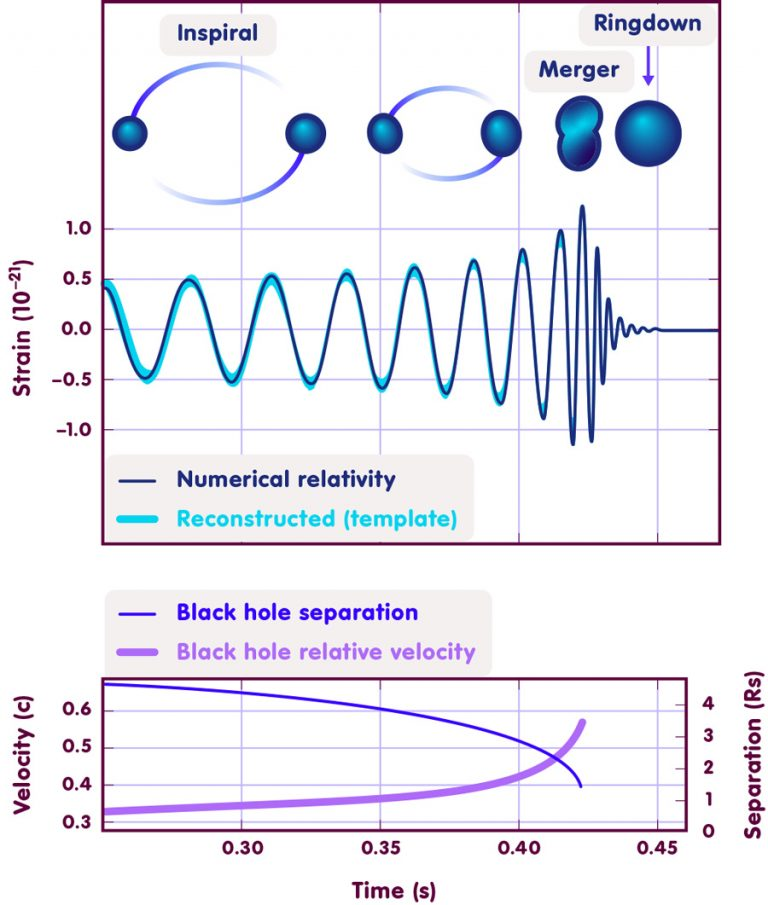
\includegraphics[height=0.8\textwidth, width=0.7\textwidth]{images/grav_wave_graph.jpg}
\caption{\small Estimated gravitational wave amplitude of GW150914 at the Hanford detector. Above that are the Schwarzschild horizons of both merging black holes shown as calculated numerically from the general theory of relativity. Below: The effective distance of the black holes in units of Schwarzschild radii RS and the relative velocity in units of the speed of light. [Image: LIGO / Redesign: Daniela Leitner]}
\end{figure}

Magnetar-driven shock breakouts (SBOs) can provide crucial electromagnetic (EM) triggers for GW searches of long-transients emitted by newly formed magnetars. They will help enhance the sensitivity of GW searches in two complementary ways: on the one hand by providing the start time for the transient signal, and on the other hand by constraining the NS spin period and B-field, which in turn determine the GW signal shape.\\

Magnetar-driven SBOs detected by ULTRASAT will have for the joint search of GW long transients emitted by newly born magnetars. Not only will magnetardriven SBOs represent a necessary EM trigger for GW searches, but they will also provide direct constraints on the GW signal parameters. Both factors will contribute to improving the sensitivity of GW searches, hence extending their horizon and the expected event rate (0.1  $ yr^{-1}$).\citeauthorandyear{Magnetar_GW}\\




\newpage\\
\section{Conclusion}

We have provided a brief overview of neutron stars, their types, and the processes involved in their formation, analysis of their GW waves in this review study. We have covered Black Widow Pulsars and Magnetars, two unique varieties of neutron stars. We discussed the radius, density, rotational speed, surface temperature, and escape velocity of neutron stars, among other characteristics. We can learn more about the makeup of neutron stars by analysing the gravitational waves that high magnetic neutron stars release, known as Continuous Gravitational Waves. It is still unknown how magnetars and black widow pulsars are formed. Continuous gravitational waves can be used to approximate neutron star parameters, such as their mass, radius etc. which will help us characterise stars as they get closer to becoming one of the different types of neutron stars and understand the structure and makeup of Magnetar and other families of neutron stars. The first continuous observation of gravitational waves would be a significant scientific discovery. However, what we learn as a result of that discovery may be even more astounding.


\newpage
\printbibliography

\end{document}